
\documentclass[9pt]{beamer}

\usepackage{inputenc}
\usepackage[T1]{fontenc}
\usepackage{textcomp}
\usepackage{amsmath}
\usepackage{amsthm}
\usepackage{amssymb}
\usepackage{euler}
\usepackage{fontspec}
\usepackage{minted}
\usepackage{graphicx}
\usepackage{fancyvrb}
\usepackage{bbold}

\usetheme[titleformat=smallcaps,block=fill]{metropolis}

%\renewcommand{\rmdefault}{eulervm}

%\usefonttheme{professionalfonts}
\setmonofont[Scale=0.8]{Menlo}
%\usefonttheme[onlymath]{serif}

\usemintedstyle{xcode}

\setbeamertemplate{blocks}[rounded]

%Information to be included in the title page:
\title{My PhD $3$rd year summary}
\author{Massimo Nocentini}
\institute{University of Florence, Italy}
\date{\today}

\begin{document}

\frame{\titlepage}


\begin{frame}[fragile]
\frametitle{}
\begin{minted}[escapeinside=||,mathescape=true]{smalltalk}
outline
    ^ LinkedList new
        add: 'me, seminars and conferences';
        add: 'what you (already?) know about my work';
        add: 'mining the OEIS';
        add: 'matrices functions';
        add: '|$\mu$|Kanren into HOL Light'; 
        yourself
\end{minted}
\end{frame}


\begin{frame}[fragile]
\frametitle{Hi, again!}
\begin{Verbatim}
$ whoami
Massimo Nocentini
PhD student @ University of Florence
Mathematician (algebraic combinatorics, formal methods for algs)
Programmer (automated reasoning, logics and symbolic comp)
https://github.com/massimo-nocentini (50 public repos)
$ clear
\end{Verbatim}

\begin{block}{Seminars and Conferences}
\begin{itemize}
\item September, 2018: $\mu$Kanren in Smalltalk, speaker @ ESUG
\item April, 2018: \textit{<Programming>} conf, participant @ Nice
\item November, 2017: $\mu$Kanren in Python, speaker @ Logic Dep 
\end{itemize}
\end{block}

\end{frame}


\begin{frame}[fragile]
\frametitle{what you know about my work}

Languages $\mathfrak{L}^{[\mathfrak{p}]}\subset \{0,1\}^*$ of binary words $w$
avoiding a \textit{Riordan pattern} $\mathfrak{p}$ are enumerated,
wrt $1$-bits and $0$-bits, by
$$F^{[\mathfrak{p}]}(x,y)
=\genfrac{}{}{1pt}{0}{C^{[\mathfrak{p}]}(x,y)}{(1-x-y)C^{[\mathfrak{p}]}(x,y)
+x^{n_1^{[\mathfrak{p}]}}y^{n_0^{[\mathfrak{p}]}}}$$
Let $R_{n,k}^{[\mathfrak{p}]}$ be the number of words avoiding $\mathfrak{p}$
and having $n$ $1$-bits  and $n-k$  $0$-bits, formally 
${\mathcal{F}_{n,k}^{[\mathfrak{p}]}} = {\mathcal{R}_{n,
n-k}^{[\bar{\mathfrak{p}]}}}$; moreover, let
$\mathcal{R}^{[\mathfrak{p}]}=\left(R_{n,k}^{[\mathfrak{p}]}\right)_{n,k\in\mathbb{N}}$
be the enclosing matrix and ${\cal{R}^{[\mathfrak{p}]}}$ is a
\textit{Riordan array} if and only if  $\mathfrak{p}$ is a Riordan pattern.
\vfill
\noindent\rule{\textwidth}{0.1pt}
{\footnotesize
Merlini \& Nocentini. \textit{Algebraic Generating Functions for Languages
Avoiding Riordan Patterns}.  Journal of Integer Sequences, 2018.}
\end{frame}

\begin{frame}[fragile]
\frametitle{what you know about my work}

Let $\mathfrak{p}$ be a Riordan pattern
such that $n_1^{[\mathfrak{p}]}-n_0^{[\mathfrak{p}]}=1$, then
$\mathcal{R}^{\left[\mathfrak{p}\right]}$ is defined by
$$d^{[\mathfrak{p}]}(t)={C^{[\mathfrak{p}]}(t)
\over \sqrt{C^{[\mathfrak{p}]}(t)^2-4tC^{[\mathfrak{p}]}(t)(C^{[\mathfrak{p}]}(t)-t^{n_0^{[\mathfrak{p}]}})}}\quad\text{and}$$
$$h^{[\mathfrak{p}]}(t)={C^{[\mathfrak{p}]}(t) -\sqrt{C^{[\mathfrak{p}]}(t)^2-4tC^{[\mathfrak{p}]}(t)(C^{[\mathfrak{p}]}(t)-t^{n_0^{[\mathfrak{p}]}})}
\over 2 C^{[\mathfrak{p}]}(t)},$$
where $C^{[\mathfrak{p}]}(t)=C^{[\mathfrak{p}]}(\sqrt{t},\sqrt{t})$.
\vfill
\noindent\rule{\textwidth}{0.1pt}
{\footnotesize
Merlini \& Nocentini. \textit{Algebraic Generating Functions for Languages
Avoiding Riordan Patterns}.  Journal of Integer Sequences, 2018.}
\end{frame}

\begin{frame}[fragile]
\frametitle{what you know about my work}

Add the constraint $|w|_0\leq |w|_1$, for any $w\in \mathfrak{L}^{[\mathfrak{p}]}$.
\begin{itemize}
\item $S^{[\mathfrak{p}]}(t)$ enumerates $\left\lbrace w\in \lbrace 0,1 \rbrace^{*}:
|w|_0\leq |w|_1\right\rbrace$ avoiding $\mathfrak{p}$\newline according to
\textit{the number of $1$-bits},
$$S^{[\mathfrak{p}]}(t)={2C^{[\mathfrak{p}]}(t) \over \sqrt{Q(t)}\left(\sqrt{C^{[\mathfrak{p}]}(t)}+ \sqrt{Q(t)} \right)} $$
    where $Q(t)={(1-4t)C^{[\mathfrak{p}]}(t)^2+4t^{n_1^{[\mathfrak{p}]}}}.$
\item $L^{[\mathfrak{p}]}(t)$ enumerates $\left\lbrace w\in \lbrace 0,1 \rbrace^{*}:
|w|_0\leq |w|_1\right\rbrace$ avoiding $\mathfrak{p}$\newline according to
\textit{the word length},
$$L^{[\mathfrak{p}]}(t)= {2tC^{[\mathfrak{p}]}(t^2)^2 \over \sqrt{Q(t)}\left((2t-1)C(t^2)+ \sqrt{ Q(t) } \right)}$$
where $Q(t)=C^{[\mathfrak{p}]}(t^2)\left( (1-4t^2)C^{[\mathfrak{p}]}(t^2)+4t^{2n_1^{[\mathfrak{p}]}}\right).$
\end{itemize}
\vfill
\noindent\rule{\textwidth}{0.1pt}
{\footnotesize
Merlini \& Nocentini. \textit{Algebraic Generating Functions for Languages
Avoiding Riordan Patterns}.  Journal of Integer Sequences, 2018.}
\end{frame}

\begin{frame}[fragile]
\frametitle{what you know about my work}

\begin{minted}[baselinestretch=0.8]{python}
"""
*      * * *   
*          *   
* * *      *   
"""
V_shape = shape_spec(name='V', isomorphisms=lambda r, c: [
                ((r,c), (r+1,c),  (r+2,c),   (r+2, c+1), (r+2, c+2)),
                ((r,c), (r, c+1), (r,c+2),   (r+1, c+2), (r+2, c+2)), ])

# define here more shapes wrt the anchor position (r,c)

dim = (6,10)
tilings = polyominoes(
    dim, shapes,
    availables={s.name:3 for s in shapes},
    forbidden=[(0,0), (1,0), (2,0), (3,0), (4,0),
               (1,9), (2,9), (3,9), (4,9), (5,9),
               (1,5), (2,4), (2,5), (3,4), (3,5)])
\end{minted}
\end{frame}

\begin{frame}[fragile]
\frametitle{what you know about my work}
\begin{Verbatim}[baselinestretch=0.1, fontsize=\footnotesize]
┌─────────────────────┐   ┌─────────────────────┐
│   γ γ γ δ δ δ ζ ζ ζ │   │   γ γ γ ι ι ι ι λ λ │
│   ι ι γ δ   δ λ ζ   │   │   μ μ γ ι   ε λ λ   │
│   ι μ γ     λ λ ζ   │   │   μ μ γ     ε ε λ   │
│   ι μ μ     η λ λ   │   │   δ μ δ     η ε ε   │
│   ι μ μ θ θ η η η   │   │   δ δ δ θ θ η η η   │
│ β β β β β θ θ θ η   │   │ β β β β β θ θ θ η   │
└─────────────────────┘   └─────────────────────┘
┌─────────────────────┐   ┌─────────────────────┐
│   γ γ γ ι ι ι ι λ λ │   │   γ γ γ θ θ δ δ λ λ │
│   γ μ μ ι   ε λ λ   │   │   γ θ θ θ   δ λ λ   │
│   γ μ μ     ε ε λ   │   │   γ ε ε     δ δ λ   │
│   δ μ δ     η ε ε   │   │   ε ε κ     ζ μ μ   │
│   δ δ δ θ θ η η η   │   │   ε κ κ κ κ ζ μ μ   │
│ β β β β β θ θ θ η   │   │ β β β β β ζ ζ ζ μ   │
└─────────────────────┘   └─────────────────────┘
\end{Verbatim}
manipulation via \textit{bitmasking} techniques, the board itself $\in\mathbb{N}$...
\end{frame}

\begin{frame}[fragile]
\frametitle{what you know about my work}
\begin{Verbatim}[baselinestretch=0.5, fontsize=\footnotesize]
 ▢ ▢ ▢    ▢ ▢ ▢      ▢ ▢        ▢ ▢        ▢ ▢ ▢ ▢    ▢ ▢ ▢
 ▢ ▢ ▢    ▢ ▢ ▢      ▢ ▢ ▢      ▢ ▢        ▢ ▢ ▢ ▢    ▢ ▢ ▢
 ▢ ▢ ▢      ▢ ▢      ▢ ▢ ▢      ▢ ▢                       ▢
                                ▢ ▢


 ▢ ▢ ▢    ▢ ▢        ▢ ▢        ▢          ▢          ▢ ▢
   ▢ ▢    ▢ ▢        ▢ ▢ ▢      ▢ ▢ ▢      ▢ ▢        ▢ ▢
   ▢ ▢    ▢ ▢ ▢        ▢ ▢      ▢ ▢ ▢      ▢ ▢        ▢ ▢
                                           ▢ ▢          ▢


 ▢ ▢ ▢    ▢ ▢ ▢      ▢ ▢        ▢ ▢ ▢      ▢ ▢        ▢
   ▢ ▢    ▢ ▢ ▢ ▢    ▢ ▢          ▢ ▢      ▢ ▢ ▢      ▢ ▢
                       ▢ ▢          ▢          ▢      ▢ ▢ ▢


 ▢        ▢ ▢        ▢          ▢ ▢ ▢      ▢ ▢        ▢ ▢ ▢ ▢
 ▢ ▢ ▢      ▢ ▢      ▢ ▢          ▢ ▢ ▢    ▢ ▢ ▢ ▢        ▢ ▢
   ▢ ▢      ▢ ▢      ▢ ▢
                       ▢


 ▢ ▢      ▢          ▢ ▢ ▢      ▢          ▢          ▢ ▢
 ▢ ▢      ▢              ▢      ▢ ▢        ▢ ▢ ▢        ▢
   ▢      ▢ ▢            ▢        ▢ ▢          ▢        ▢ ▢
   ▢      ▢ ▢


 ▢ ▢      ▢          ▢          ▢ ▢        ▢          ▢ ▢ ▢
   ▢ ▢    ▢          ▢ ▢ ▢ ▢      ▢        ▢              ▢ ▢
     ▢    ▢ ▢ ▢                   ▢        ▢
                                  ▢        ▢ ▢


 ▢        ▢ ▢ ▢ ▢    ▢          ▢ ▢        ▢          ▢ ▢ ▢ ▢ ▢
 ▢              ▢    ▢ ▢          ▢ ▢ ▢    ▢
 ▢ ▢                   ▢                   ▢
   ▢                   ▢                   ▢
                                           ▢
\end{Verbatim}
The set of \textit{parallelogram polyominoes} of semi-perimeter $6$
\end{frame}

\begin{frame}[fragile]
\frametitle{what you know about my work}
We have a generator of \textit{parallelogram polyominoes} of arbitrary
semi-perimeter; moreover, pps can be use to tile square boards
\vfill
\begin{Verbatim}[baselinestretch=0.1, fontsize=\footnotesize]
 _ _ _ _ _ _ _ _ _ _ _ _ _ _ _       _ _ _ _ _ _ _ _ _ _ _ _ _ _ _ _
|     |   | |_    |_ _ _ _ _| |●    |     |   | |_    | |_  |_ _    |
|     |   |   |_  |   |   | |   |   |     |   |   |_  |   |_ _ _|_ _|
|_ _ _|   |   | |_|_  |   | |_  |   |_ _ _|   |   | |_|_ _ _|_ _ _  |
|     |_ _|_ _|_    | |_  | | |_|   |     |_ _|_ _|_    |   | |_  |_|
|_    |     |   |_ _|_| |_| | |●    |_    |     |   |_ _|   | | |   |
| |_ _|_ _  |_  |_    |_  |_|   |   | |_ _|_ _  |_  | | |_  | | |_ _|
|     |   |_| |_ _|_ _ _|_ _|_ _|   |     |   |_| | | |_  |_| | |_  |
|_ _ _|_ _  |   |_  |_  |_  | |●    |_ _ _|_ _  | |_|_  |_ _|_|_ _| |
|   |_    |_|_ _ _|_  |   | |_  |   |   |_    |_|_ _ _|_| |_  |   | |
|     |   |     |_  |_|_ _|_ _| |   |     |   |     |_  |_  | |_  |_|
|_ _ _|_ _|_ _ _ _|_ _ _|_  | |_|   |_ _ _|_ _|_ _ _ _|_  | |_ _|_ _|
|       |_      |   |_ _  | | |●    |       |_      |   |_|_| |_ _  |
|_ _ _ _| |_ _ _|_ _ _ _| | | |●    |_ _ _ _| |_ _ _|_ _ _ _|   | | |
|   |   |_ _  |_ _ _  | |_|_|_ _|   |   |   |_ _  |_ _ _ _ _|_  | |_|
|   |_    | |_|_ _  |_| |_ _    |   |   |_    | |_|_ _  |_    |_|   |
|_ _ _|_ _|_ _ _ _|_ _|_ _ _|_ _|   |_ _ _|_ _|_ _ _ _|_ _|_ _ _|_ _|
\end{Verbatim}
\end{frame}


\begin{frame}[fragile]
\frametitle{what you (already?) know about my work}
\begin{columns}
\begin{column}{0.6\textwidth}
the Big Beng
\begin{Verbatim}[baselinestretch=0.5,fontsize=\footnotesize]
            ★
\end{Verbatim}
the (i) generation
\begin{Verbatim}[baselinestretch=0.5,fontsize=\footnotesize]
            ●
           ★ ★
\end{Verbatim}
the (ii) generation
\begin{Verbatim}[baselinestretch=0.5,fontsize=\footnotesize]
         ●     ●
        ● ★     ●
       ★ ★     ★ ★
\end{Verbatim}
the (iii) generation
\begin{Verbatim}[baselinestretch=0.5,fontsize=\footnotesize]
   ●      ●      ●      ●     ●
  ● ★    ● ★    ● ●      ●     ●
 ● ★      ●      ★ ★    ● ★     ●
★ ★      ★ ★           ★ ★     ★ ★
\end{Verbatim}
the (iv) generation
\begin{Verbatim}[baselinestretch=0.5,fontsize=\footnotesize]
    ●       ●        ●        ●       ●     
   ● ★     ● ★      ● ★      ● ●       ●    
  ● ★     ● ★      ● ●      ● ★ ★       ●   
 ● ★       ●        ★ ★                ● ★  
★ ★       ★ ★                         ★ ★   

  ●       ●         ●          ●      ●
 ● ★     ● ●       ●          ● ●      ●
  ●       ☆ ★       ●          ● ★      ●
 ● ★       ★         ●        ★ ★        ●
★ ★                 ★ ★                 ★ ★

 ●          ●        ●         ●
● ●          ●        ●         ●
   ●        ● ★      ● ★       ● ●
  ★ ★      ● ★        ●         ★ ★
          ★ ★        ★ ★
\end{Verbatim}
\end{column}
\begin{column}{0.4\textwidth}  %%<--- here
An implementation of the ECO methodology to represent \textit{recursive
structure}; for instance, on the left is shown the enumeration of
\textit{binary trees}, defined according to the symbolic equation
\begin{Verbatim}[baselinestretch=0.5,fontsize=\footnotesize]
★  =   ●
      ★ ★
\end{Verbatim}
\end{column}
\end{columns}
\end{frame}

\begin{frame}[fragile]
\frametitle{Mining the OEIS: an extended grapher}
\begin{figure}
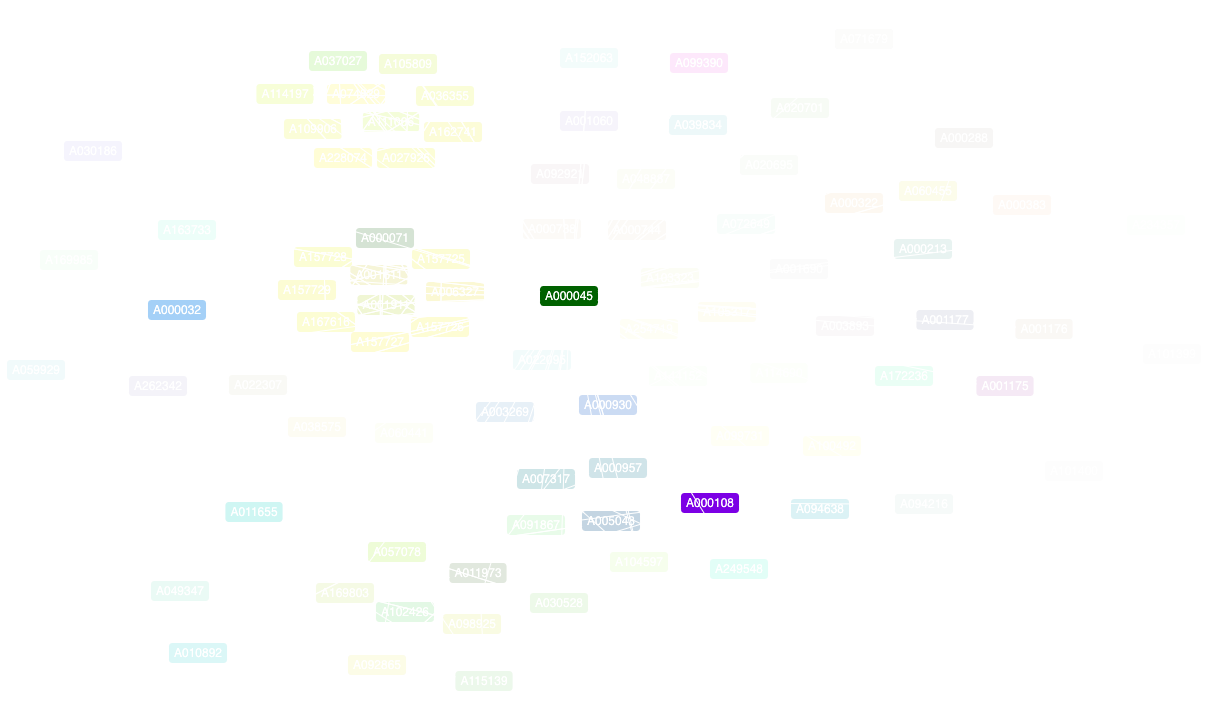
\includegraphics[width=12cm,height=8cm]{coloured}
\iffalse
\caption{Sequences network with labelel vertices, here we see that the sequence
of \textit{Fibonacci numbers} (\url{https://oeis.org/A000045}) and of
\textit{Catalan numbers} (\url{https://oeis.org/A000108}) are the two central
sequences, respectively.}
\fi
\end{figure}
\end{frame}

\begin{frame}[fragile]
\frametitle{Functions of Riordan matrices}
\begin{columns}
    \begin{column}{0.6\textwidth}
        \begin{displaymath}
        \footnotesize
        %\mathcal{P}_{8}=\left[\begin{matrix}1 &   &   &   &   &   &   &  \\1 & 1 &   &   &   &   &   &  \\1 & 2 & 1 &   &   &   &   &  \\1 & 3 & 3 & 1 &   &   &   &  \\1 & 4 & 6 & 4 & 1 &   &   &  \\1 & 5 & 10 & 10 & 5 & 1 &   &  \\1 & 6 & 15 & 20 & 15 & 6 & 1 &  \\1 & 7 & 21 & 35 & 35 & 21 & 7 & 1\end{matrix}\right]
        \mathcal{C}_{8}=\left[\begin{matrix}1 &   &   &   &   &   &   &  \\1 & 1 &   &   &   &   &   &  \\2 & 2 & 1 &   &   &   &   &  \\5 & 5 & 3 & 1 &   &   &   &  \\14 & 14 & 9 & 4 & 1 &   &   &  \\42 & 42 & 28 & 14 & 5 & 1 &   &  \\132 & 132 & 90 & 48 & 20 & 6 & 1 &  \\429 & 429 & 297 & 165 & 75 & 27 & 7 & 1\end{matrix}\right]
        \end{displaymath}
        \begin{displaymath}
        \footnotesize
        e^{\mathcal{C}_{8}} = e \left[\begin{matrix}1 &   &   &   &   &   &   &  \\1 & 1 &   &   &   &   &   &  \\3 & 2 & 1 &   &   &   &   &  \\\frac{23}{2} & 8 & 3 & 1 &   &   &   &  \\\frac{154}{3} & 37 & 15 & 4 & 1 &   &   &  \\\frac{1 27}{4} & \frac{572}{3} & \frac{163}{2} & 24 & 5 & 1 &   &  \\\frac{7 46}{5} & \frac{6439}{6} & 478 & 15  & 35 & 6 & 1 &  \\\frac{5 2481}{6 } & \frac{39 899}{6 } & \frac{12  5}{4} & \frac{2965}{3} & \frac{495}{2} & 48 & 7 & 1\end{matrix}\right]
        \end{displaymath}
    \end{column}
    \begin{column}{0.4\textwidth}
    Lift the scalar function $$f: \mathbb{R} \rightarrow \mathbb{R}$$
    to the matrix function
    $$\hat{f}: \mathbb{R}^{m\times m} \rightarrow \mathbb{R}^{m\times m}$$
    where $m\in\mathbb{N}$, provided that
    \begin{displaymath}
        \left. \frac{\partial^{(j)}{f}}{\partial{z}^{j}} \right|_{z=\lambda_{i}},\,
        \begin{array}{l} 
            i\in \lbrace 1, \ldots, \nu \rbrace \\
            j \in \lbrace 0, \ldots, m_{i}-1 \rbrace
        \end{array},
    \end{displaymath}
    exists, for each eigenvalue $\lambda_{i}$.
    \end{column}
\end{columns}
\vfill
\noindent\rule{\textwidth}{0.1pt}
{\footnotesize
Merlini \& Nocentini. \textit{Functions and Jordan Canonical Forms of Riordan
matrices}. \newline Linear Algebra and its Applications, under review.}
\end{frame}

\begin{frame}[fragile]
\frametitle{Functions of Riordan matrices}
\begin{displaymath}
\footnotesize
    \sqrt[3]{\mathcal{P}_{8}}= \left[\begin{matrix}1 &  &  &  &  &  &  & \\\frac{1}{3} & 1 &  &  &  &  &  & \\\frac{1}{9} & \frac{2}{3} & 1 &  &  &  &  & \\\frac{1}{27} & \frac{1}{3} & 1 & 1 &  &  &  & \\\frac{1}{81} & \frac{4}{27} & \frac{2}{3} & \frac{4}{3} & 1 &  &  & \\\frac{1}{243} & \frac{5}{81} & \frac{10}{27} & \frac{10}{9} & \frac{5}{3} & 1 &  & \\\frac{1}{729} & \frac{2}{81} & \frac{5}{27} & \frac{20}{27} & \frac{5}{3} & 2 & 1 & \\\frac{1}{2187} & \frac{7}{729} & \frac{7}{81} & \frac{35}{81} & \frac{35}{27} & \frac{7}{3} & \frac{7}{3} & 1\end{matrix}\right]
\end{displaymath}
such that %$\sqrt{\mathcal{P}_8} \cdot \sqrt{\mathcal{P}_8} =\mathcal{P}_8$ and
$\sqrt[3]{\mathcal{P}_8} \cdot \sqrt[3]{\mathcal{P}_8} \cdot
\sqrt[3]{\mathcal{P}_8} =\mathcal{P}_8$ and
$L_{8}\left({e^{\mathcal{C}_{8}}}\right) = \mathcal{C}_{8}$, where polynomial
\begin{displaymath}
{L_{ 8 }}{\left (z \right )} = \frac{z^{7}}{7 e^{7}} - \frac{7 z^{6}}{6 e^{6}} + \frac{21 z^{5}}{5 e^{5}} - \frac{35 z^{4}}{4 e^{4}} + \frac{35 z^{3}}{3 e^{3}} - \frac{21 z^{2}}{2 e^{2}} + \frac{7 z}{e} - \frac{223}{140}
\end{displaymath}
interpolates the $log$ function; moreover, the classic identity 
$$sin(\mathcal{P}_8)\cdot sin(\mathcal{P}_8)+
cos(\mathcal{P}_8)\cdot cos(\mathcal{P}_8)=I_{8},$$ 
where $I$ is the identity matrix, holds as well.
\vfill
\noindent\rule{\textwidth}{0.1pt}
{\footnotesize
Merlini \& Nocentini. \textit{Functions and Jordan Canonical Forms of Riordan
matrices}. \newline Linear Algebra and its Applications, under review.}
\end{frame}

\begin{frame}[fragile]
\frametitle{Functions of Riordan matrices}
Generalized Lagrange bases and Hermite interpolating polys
\begin{columns}
    \begin{column}{0.5\textwidth}
        \begin{displaymath}
        \footnotesize
        \left. \frac{\partial^{(r-1)}{\Phi_{i,j}}}{\partial{z}^{r-1}} \right|_{z=\lambda_{l}} = \delta_{i,l}\delta_{j,r},
        \, 
        \begin{array}{l} 
            l\in \lbrace 1, \ldots, \nu \rbrace \\
            r \in \lbrace 1, \ldots, m_{l} \rbrace
        \end{array}
        \end{displaymath}
        \begin{displaymath}
        \footnotesize
        g(z) = \sum_{i=1}^{\nu}{\sum_{j=1}^{m_{i}}{ \left.
        \frac{\partial^{(j-1)}{f}}{\partial{z}^{j-1}} \right|_{z=\lambda_{i}}\Phi_{i,j}(z) }}
        \end{displaymath}
    \end{column}
    \vrule{}
    \begin{column}{0.5\textwidth}
        \begin{displaymath}
        \footnotesize
          \Phi_{1,j}(z) = \frac{\left(z-\lambda_{1}\right)^{j-1}}{(j-1)!}, 
          \, j\in \lbrace 1,\ldots, m_{1} \rbrace
        \end{displaymath}
        \begin{displaymath}
        \footnotesize
        g_{m}(z) = {\sum_{j=1}^{m}{ \left.
        \frac{\partial^{(j-1)}{f}}{\partial{z}^{j-1}} \right|_{z=\lambda_{1}}}}
        \frac{\left(z-\lambda_{1}\right)^{j-1}}{(j-1)!}
        \end{displaymath}
    \end{column}
\end{columns}
for \textit{arbitrary} and \textit{Riordan} matrices, respectively.
We study functions
\begin{displaymath}
\begin{split}
f(z)&=z^{r},\,{f(z)=\frac{1}{z}},\,{f(z)=\sqrt{z}},\,{f(z)=e^{\alpha z}},\\
f(z)&=log\,{z},\,f(z)=sin\,{z}\quad\text{and}\quad f(z)=cos\,{z},
\end{split}
\end{displaymath}
applying them to Riordan matrice $\mathcal{P}_{8}$, $\mathcal{C}_{8}$ and 
$\mathcal{S}_{8}$.
\vfill
\noindent\rule{\textwidth}{0.1pt}
{\footnotesize
Merlini \& Nocentini. \textit{Functions and Jordan Canonical Forms of Riordan
matrices}. \newline Linear Algebra and its Applications, under review.}
\end{frame}

\begin{frame}[fragile]
\frametitle{Functions of Riordan matrices}
\begin{columns}
    \begin{column}{0.35\textwidth}
        \begin{displaymath}
        \begin{split}
          P_{m}(z) &= \sum_{j=0}^{m-1}{\binom{r}{j}}{(z-1)^{j} }\\
          I_{m}(z) &= \sum_{j=0}^{m-1}{(-1)^{j}\,\left(z-1\right)^{j}}\\
          R_{m}(z) &= \sum_{j=0}^{m-1}{{\frac{1}{2} \choose j}\left(z-1\right)^{j}}\\
          E_{m}(z) &= e^{\alpha} \sum_{j=0}^{m-1}{\frac{\alpha^{j}}{j!}\left(z-1\right)^{j}}\\
          L_{m}(z) &= \sum_{j=1}^{m-1}{\frac{(-1)^{j-1}}{j}{\left(z-1\right)^{j} }}\\
        \end{split}
        \end{displaymath}
    \end{column}
    \vrule{}
    \begin{column}{0.65\textwidth}
        \begin{displaymath}
        \footnotesize
        \begin{split}
          S_{m}(z)  &= sin\,{1}\,\sum_{k=0}^{2\,\left\lceil \frac{m}{2} \right\rceil-2}{\left(\sum_{j=\left\lceil \frac{k}{2}\right\rceil}^{\left\lceil \frac{m}{2} \right\rceil -1}{\frac{(-1)^{3j}}{(2j)!}{2j\choose k}}\right) {(-z)^{k}}}\\
                    &+ cos\,{1}\,\sum_{k=0}^{2\,\left\lfloor \frac{m}{2} \right\rfloor-1}{\left(\sum_{j=\left\lfloor \frac{k}{2}\right\rfloor}^{\left\lfloor \frac{m}{2} \right\rfloor -1}{\frac{(-1)^{3j+1}}{(2j + 1)!} {2j+1\choose k}}\right){(-z)^{k}}}\\
          C_{m}(z)  &= cos\,{1}\,\sum_{k=0}^{2\,\left\lceil \frac{m}{2} \right\rceil-2}{\left(\sum_{j=\left\lceil \frac{k}{2}\right\rceil}^{\left\lceil \frac{m}{2} \right\rceil -1}{\frac{(-1)^{3j}}{(2j)!}{2j\choose k}}\right) {(-z)^{k}}}\\
                    &+ sin\,{1}\,\sum_{k=0}^{2\,\left\lfloor \frac{m}{2} \right\rfloor-1}{\left(\sum_{j=\left\lfloor \frac{k}{2}\right\rfloor}^{\left\lfloor \frac{m}{2} \right\rfloor -1}{\frac{(-1)^{3j+2}}{(2j + 1)!} {2j+1\choose k}}\right){(-z)^{k}}}\\
        \end{split}
        \end{displaymath}
    \end{column}
\end{columns}
where $c\cdot(d_{n,k})_{n,k\in\mathbb{N}} = (c\cdot d_{n,k})_{n,k\in\mathbb{N}}$.
\vfill
\noindent\rule{\textwidth}{0.1pt}
{\footnotesize
Merlini \& Nocentini. \textit{Functions and Jordan Canonical Forms of Riordan
matrices}. \newline Linear Algebra and its Applications, under review.}
\end{frame}

\iffalse

\begin{frame}[fragile]

\frametitle{Resolution by \textit{Refutation}}

Let $\alpha$ be a sentence in \textit{CNF} and $M(\alpha)$ the set of models that
satisfy it, where a model is a set of assignments that make $\alpha$ true.
\vfill
$\alpha$ is \textit{valid} if it is true in \textit{all} models; oth,\\
$\alpha$ is \textit{satisfiable} if it is true in \textit{some} model.
\vfill
Let $\models$ and $\Rightarrow$ denote the \textit{entail} and \textit{imply} relations, respectively, in
\begin{displaymath}
\begin{split}
\alpha &\models \beta \leftrightarrow \\
M(\alpha) &\subseteq M(\beta) \leftrightarrow \\
(\alpha &\Rightarrow \beta) \text{ is valid } \leftrightarrow\\
\neg(\neg\alpha &\vee \beta) \text{ is unsatisfiable;}
\end{split}
\end{displaymath}
therefore, to prove a sentence $\alpha$ reduces to decide
$$\neg\alpha\models\perp\quad\leftrightarrow\quad\alpha\text{ is valid,}$$
where $\perp$ denotes the empty clause, namely \textit{falsehood}.
\end{frame}

\begin{frame}[fragile]
\frametitle{Resolution by \textit{Refutation}}
The \textit{resolution rule} is a \textit{complete} inference algorithm,
\begin{displaymath}
{\left(l_{0}, \ldots, l_{i}, \ldots, l_{j-1}\right) \quad \left(m_{0}, \ldots, m_{r},\ldots, m_{k-1}\right) \quad l_{i} = \neg m_{r}
\over
\left(l_{0},\ldots, l_{i-1},l_{i+1}, \ldots,l_{j-1}, m_{0},\ldots, m_{r-1},m_{r+1},\ldots, m_{k-1}\right)}
\end{displaymath}
where $\left(l_{0},\ldots, l_{i}, \ldots, l_{j-1}\right) = l_{0}\vee \ldots
\vee l_{i} \vee \ldots \vee l_{j-1}$, \\
for all $l_{q}, m_{w} \in\lbrace 0,1\rbrace$.
\vfill
The \textit{DPLL} algorithm is a recursive, depth-first enumeration of models
using the resolution rule, paired with heuristics \textit{early termination},
\textit{pure symbol} and \textit{unit clause} to speed up.
\end{frame}

\begin{frame}[fragile]
\frametitle{Resolution by \textit{Unification}}

\textit{Unification} is the process of solving \textit{equations among symbolic
expressions}; a \textit{solution} is denoted as a \textit{substitution}
$\theta$, namely a mapping that assigns a symbolic values to free variables.
\vfill
Let $x$ and $y$ be free variables, the set
$$\lbrace cons(x,cons(x,nil)) = cons(2,y)\rbrace$$
has solution $\theta = \lbrace x \mapsto 2, y \mapsto cons(2,nil) \rbrace$;
moreover, the set
$$ \lbrace y = cons(2,y) \rbrace $$
has no \textit{finite} solution; on the other hand,
$$\theta = \lbrace y \mapsto cons(2,cons(2,cons(2,...))) \rbrace$$
is a solution upto \textit{bisimulation}.
\end{frame}

\begin{frame}[fragile]
\frametitle{Resolution by \textit{Unification}}
let $G$ be a set of equations, unification rules are
\begin{description}
\item[delete] $G \cup \lbrace t = t \rbrace \rightarrow G$
\item[decompose] $G \cup \lbrace f(s_{0}, \ldots, s_{k}) = f(t_{0}, \ldots, t_{k})\rbrace$ entails
$$G \cup \lbrace s_{0}=t_{0},\ldots, s_{k}=t_{k} \rbrace$$
\item[conflict] if $f\neq g \vee k\neq m$ then $$G \cup \lbrace f(s_{0}, \ldots, s_{k}) = g(t_{0}, \ldots, t_{m})\rbrace \rightarrow \,\perp$$
\item[eliminate] if $x \not\in vars(t)$ and $x \in vars(G)$ then $$G \cup \lbrace x = t\rbrace \rightarrow G\lbrace x \mapsto t\rbrace \cup \left\lbrace x \triangleq t\right\rbrace $$
\item[occur check] if $x \in vars(f(s_{0},\ldots,s_{k}))$ then $$G \cup \lbrace x = f(s_{0}, \ldots, s_{k})\rbrace \rightarrow \,\perp$$
\end{description}
%without *occur checks*, generating a substitution $\theta$ is a *recursive enumerable* problem
\end{frame}

\begin{frame}[fragile]
\frametitle{microkanren}
Let \textit{solution}, \textit{substitution} and \textit{state} be synonyms; so, $\mu$-kanren
\begin{itemize}
\item is a \textit{DSL} for relational programming written in Scheme
\item is a \textit{purely functional} core of \textit{miniKanren}
\item provides \textit{explicit streams} of satisfying states
\item encodes math rel using a \textit{goal-based} approach
\item uses resolution by unification via \textit{structural induction}
\end{itemize}
\vfill
A \textit{goal} is an object that responds to the \verb|#onState:| selector, it
receives a \textit{substitution} and returns a \verb|Chain| object of
substitutions.
\end{frame}

\begin{frame}[fragile]
\frametitle{Chain hierarchy}
We model a (possibly infinite) space of objects with the
\verb|Chain| hierarchy, which has \verb|Bottom| and \verb|Knot|
as subclasses which denote the empty and a populated set, respectively.
\vfill
Although Pharo provides the \verb|Generator| class, we write our version of
\textit{lazy} enumeration, which is purely functional (neither clever uses of
\verb|thisContext| nor reentrant blocks).
\vfill
Encodes the two \textit{monadic} operations \verb|mplus| and \verb|bind|,
which allow us to merge two \verb|Chain|s and to combine a \verb|Chain| obj
to yield an extended \verb|Chain| obj, respectively.
\vfill
Dispatch over two strategies \verb|Sequential| and \verb|Interleaved| in
order to \textit{enumerate} solution spaces.
\end{frame}

\begin{frame}[fragile]
\frametitle{Chain subclass: \#Bottom}

\begin{minted}[fontsize=\footnotesize]{smalltalk}
BlockClosure>>links: anObj
    ^ Chain item: anObj linker: self
\end{minted}
\begin{minted}[fontsize=\footnotesize]{smalltalk}
Chain class>>bottom
    ^ Bottom new
\end{minted}
\begin{minted}[fontsize=\footnotesize]{smalltalk}
Chain class>>item: anObj linker: aBlockClosure
    ^ Knot new
        item: anObj;
        linker: aBlockClosure;
        yourself
\end{minted}
\begin{minted}[fontsize=\footnotesize]{smalltalk}
bind: aGoal interleaved: anInterleaved
    ^ self
\end{minted}
\begin{minted}[fontsize=\footnotesize]{smalltalk}
mplus: anotherChain interleaved: anInterleaved
    ^ anotherChain value
\end{minted}
\begin{minted}[fontsize=\footnotesize]{smalltalk}
atMost: anInteger
    ^ self
\end{minted}
\begin{minted}[fontsize=\footnotesize]{smalltalk}
mature
    ^ LinkedList new
\end{minted}
\end{frame}

\begin{frame}[fragile]
\frametitle{Chain subclass: \#Knot}
\begin{minted}[fontsize=\footnotesize]{smalltalk}
bind: aGoal interleaved: anInterleaved
    | alpha beta |
    alpha := aGoal onState: item.
    beta := [ self next bind: aGoal interleaved: anInterleaved ].
    ^ alpha mplus: beta interleaved: anInterleaved
\end{minted}
\begin{minted}[fontsize=\footnotesize]{smalltalk}
mplus: anotherChain interleaved: anInterleaved
    ^ [ :_ | anotherChain value
                mplus: [ self next ]
                interleaved: anInterleaved ] links: item
\end{minted}
\begin{minted}[fontsize=\footnotesize]{smalltalk}
next
    ^ linker value: item
\end{minted}
\begin{minted}[fontsize=\footnotesize]{smalltalk}
atMost: n
    ^ n isZero
        ifTrue: [ Chain bottom ]
        ifFalse: [ [ :_ | self next value atMost: n - 1 ] links: item ]
\end{minted}
\begin{minted}[fontsize=\footnotesize]{smalltalk}
mature
    ^ self next mature
        addFirst: item;
        yourself
\end{minted}
\end{frame}

\begin{frame}[fragile]
\frametitle{ChainTest}
\begin{minted}[fontsize=\footnotesize]{smalltalk}
ints: i
    ^ [ :a | self ints: a + 1 ] links: i
\end{minted}
\begin{minted}[fontsize=\footnotesize]{smalltalk}
fib: m fib: n
    ^ [ :_ | self fib: n fib: m + n ] links: m
\end{minted}
\begin{minted}[fontsize=\footnotesize]{smalltalk}
collatz: o
    ^ [ :_ | o even
                ifTrue: [ self collatz: o / 2 ]
                ifFalse: [ self collatz: 3 * o + 1 ] ] links: o
\end{minted}
\begin{minted}[fontsize=\footnotesize]{smalltalk}
testNumbers
    self
        assert: (self nats atMost: 10) mature
        equals: (0 to: 9).
    self
        assert: (self fibs atMost: 10) mature
        equals: {0 . 1 . 1 . 2 . 3 . 5 . 8 . 13 . 21 . 34}.
    self
        assert: ((self collatz: 10) atMost: 10) mature
        equals: {10 . 5 . 16 . 8 . 4 . 2 . 1 . 4 . 2 . 1}.
\end{minted}
\end{frame}

\iffalse
\begin{frame}[fragile]
\frametitle{Chain combinators}
\begin{minted}[fontsize=\footnotesize]{smalltalk}
Bind class>>combine: aGoal with: aCollection
    ^ self new
        combiner: aGoal;
        stream: aCollection;
        yourself
\end{minted}
\begin{minted}[fontsize=\footnotesize]{smalltalk}
Bind>>interleavedStrategy: anInterleaved
    ^ stream bind: combiner interleaved: anInterleaved
\end{minted}
\begin{minted}[fontsize=\footnotesize]{smalltalk}
MPlus class>>with: aCollection with: anotherCollection
    ^ self new
        left: aCollection;
        right: anotherCollection;
        yourself
\end{minted}
\begin{minted}[fontsize=\footnotesize]{smalltalk}
MPlus>>interleavedStrategy: anInterleaved
    ^ left mplus: right interleaved: anInterleaved
\end{minted}
\begin{minted}[fontsize=\footnotesize]{smalltalk}
Sequential>>of: aStreamCombination
    ^ aStreamCombination sequentialStrategy: self
\end{minted}
\begin{minted}[fontsize=\footnotesize]{smalltalk}
Interleaved>>of: aStreamCombination
    ^ aStreamCombination interleavedStrategy: self
\end{minted}
\end{frame}
\fi

\begin{frame}[fragile]
\frametitle{Goal hierarchy}
\textit{microkanren} represents math rels using the \verb|Goal| hierarchy
\begin{itemize}
\item \verb|Succeed| it \textit{is} satisfied by \textit{each} sub;
\item \verb|Fail| it \textit{is not} satisfied by \textit{any} sub;
\item \verb|Or| it is satisfied if at least one obj it consumes can be satisfied;
\item \verb|And| it is satisfied if both objs it consumes can be satisfied;
\item \verb|Fresh| it introduces logic vars into the goal it combines;
\item \verb|Unify| it is satisfied if the two objs it consumes can be unified.
\end{itemize}
\vfill
Moreover, a substitution (aka, a set of assignments) is represented by a
\verb|Dictionary| obj, wrapped by \verb|State| obj to count the number of logic
vars introduced by \verb|Fresh| goals.
\vfill
Our substitutions are \textit{triangular} in the sense that if
\begin{displaymath}
\theta =  \lbrace x \mapsto y, y \mapsto z, z \mapsto 3 \rbrace
\end{displaymath}
then $x \mapsto 3$ is subsumed by $\theta$,
this is implemented in \mintinline{smalltalk}|State>>#walk|.
\end{frame}

\begin{frame}[fragile]
\frametitle{State}
\begin{minted}[fontsize=\footnotesize]{smalltalk}
State>>walk: anObj
    | k |
    k := anObj.
    [ k := substitution at: k ifAbsent: [ ^ k ] ] repeat
\end{minted}
A substitution is extended by
\begin{minted}[fontsize=\footnotesize]{smalltalk}
State>>at: aVar put: aValue
    | s |
    s := substitution copy.
    s
        at: aVar
        ifPresent: [ :v |
            aValue = v
                ifFalse: [ UnificationError signal ] ]
        ifAbsent: [ s at: aVar put: aValue ].
    ^ self class new
        birthdate: birthdate;
        substitution: s;
        yourself
\end{minted}
\end{frame}

\begin{frame}[fragile]
\frametitle{Goal subclass: \#[Succeed | Fail | Disj | Conj]}
In parallel, \mintinline{smalltalk}{true} and \mintinline{smalltalk}{false} have logical brothers
\begin{minted}[fontsize=\footnotesize]{smalltalk}
Succeed>>onState: aState
    ^ Chain with: aState
\end{minted}
\begin{minted}[fontsize=\footnotesize]{smalltalk}
Fail>>onState: aState
    ^ Chain bottom
\end{minted}
respectively; btw, for conjuction and disjunction we have
\begin{minted}[fontsize=\footnotesize]{smalltalk}
Disj>>onState: aState
    ^ interleaving of: ((either onState: aState)
        mplus: [ or onState: aState ])
\end{minted}
\begin{minted}[fontsize=\footnotesize]{smalltalk}
Conj>>onState: aState
    ^ interleaving of: ((both onState: aState) bind: and)
\end{minted}
\end{frame}

\begin{frame}[fragile]
\frametitle{Goal subclass: \#Fresh}
\begin{minted}[fontsize=\footnotesize]{smalltalk}
Fresh>>onState: aState
    ^ aState collectVars: (1 to: receiver numArgs) forFresh: self
\end{minted}
\begin{minted}[fontsize=\footnotesize]{smalltalk}
State>>collectVars: aCollection forFresh: aFresh
    | nextState vars |
    nextState := self class new
        substitution: substitution;
        birthdate: birthdate + aCollection size;
        yourself.
    vars := aCollection collect: [ :i | Var id: i ].
    ^ aFresh onState: nextState withVars: vars
\end{minted}
\begin{minted}[fontsize=\footnotesize]{smalltalk}
Fresh>>onState: aState withVars: aCollection
    | g |
    vars := aCollection.
    g := receiver valueWithArguments: vars.
    ^ g onState: aState
\end{minted}
\begin{minted}[fontsize=\footnotesize]{smalltalk}
BlockClosure>>fresh
    ^ Goal fresh: self
\end{minted}
\end{frame}


\begin{frame}[fragile]
\frametitle{Goal subclass: \#Unify}
\begin{minted}[fontsize=\footnotesize]{smalltalk}
Object>>unifyWith: another
    ^ Goal unify: self with: another
\end{minted}
\begin{minted}[fontsize=\footnotesize]{smalltalk}
Unify>>onState: aState
    ^ [ | extended_state |
        extended_state := Unifier new
                            unify: this with: that onState: aState.
        Goal succeed onState: extended_state ]
            on: UnificationError
            do: [ Goal fail onState: aState ]
\end{minted}
\begin{minted}[fontsize=\footnotesize]{smalltalk}
Unifier>>unify: anObj with: anotherObj onState: aState
    | aWalkedObj anotherWalkedObj |
    aWalkedObj := aState walk: anObj.
    anotherWalkedObj := aState walk: anotherObj.
    ^ aWalkedObj unifyWith: anotherWalkedObj
                 usingUnifier: self
                 onState: aState
\end{minted}
\end{frame}

\begin{frame}[fragile]
\frametitle{Unifier}
\begin{minted}[fontsize=\footnotesize]{smalltalk}
unifyObject: anObj withObject: anotherObj onState: aState
    ^ anObj = anotherObj
        ifTrue: [ aState ]
        ifFalse: [ UnificationError signal ]
\end{minted}
\begin{minted}[fontsize=\footnotesize]{smalltalk}
unifyVar: aVar withObject: anObject onState: aState
    ^ aState at: aVar put: anObject
\end{minted}
\begin{minted}[fontsize=\footnotesize]{smalltalk}
unifyVar: aVar withVar: anotherVar onState: aState
    ^ aVar = anotherVar
        ifTrue: [ aState ]
        ifFalse: [
            self unifyVar: aVar withObject: anotherVar onState: aState ]
\end{minted}
\begin{minted}[fontsize=\footnotesize]{smalltalk}
unifyLinkedList: c withLinkedList: d onState: aState
    ^ c size = d size
        ifTrue: [ (c zip: d)
            inject: aState
            into: [ :s :p | self unify: p key with: p value onState: s ] ]
        ifFalse: [ UnificationError signal ]
\end{minted}
\end{frame}


\begin{frame}[fragile]
\frametitle{Goal subclass: \#Cond}
\begin{minted}[fontsize=\footnotesize]{smalltalk}
Cond>>if: ifGoal then: thenGoal
    clauses add: ifGoal -> thenGoal
\end{minted}
\begin{minted}[fontsize=\footnotesize]{smalltalk}
Cond>>ifPure: aStrategy
    if := [ :c :o |
        IfPure new
            question: c key answer: c value otherwise: o;
            streamCombinationStrategy: aStrategy;
            yourself ]
\end{minted}
\begin{minted}[fontsize=\footnotesize]{smalltalk}
Cond>>e
    self ifPure: Sequential new
\end{minted}
\begin{minted}[fontsize=\footnotesize]{smalltalk}
Cond>>i
    self ifPure: Interleaved new
\end{minted}
\begin{minted}[fontsize=\footnotesize]{smalltalk}
Cond>>onState: aState
    | g |
    else ifNil: [ self else: false asGoal ].
    g := clauses copy
            add: else;
            reduceRight: if.
    ^ g onState: aState
\end{minted}
\end{frame}

\begin{frame}[fragile]
\frametitle{Dyck paths}
Let $\mathcal{D}$ be the set of \textit{Dyck paths} and let $\leadsto$ be the \textit{CFG}
$$
\leadsto \,= \varepsilon \,\left|\, ( \leadsto ) \leadsto \right.
$$
where $\varepsilon$ is the empty string; so, \textit{enumerate} $\mathcal{D}$
\textit{using} $\leadsto$.
\begin{minted}[fontsize=\footnotesize]{smalltalk}
dycko: alpha
    ^ Goal cond e
        if: alpha nilo then: true asGoal;
        else: [ :beta :gamma |
            (sexpTheory let: alpha
                        be: ($( cons: beta)
                        append: ($) cons: gamma)) &
            ([ self dycko: beta ] eta &
             [ self dycko: gamma ] eta) ] fresh
\end{minted}
\end{frame}

\begin{frame}[fragile]
\frametitle{Dyck paths}
\begin{minted}[fontsize=\footnotesize]{smalltalk}
testDycko
    | g |

    "enumeration"
    g := [ :alpha | combTheory dycko: alpha ] fresh.
    self
        assert: (g solutions atMost: 20)
        equals:
            ({nil . '()' . '(())' . '()()' . '(()())' . '()(())' .
            '(())()' . '()()()' . '(()()())'.  '()(()())' .
            '(())(())' . '()()(())' . '((()))' . '()(())()' .
            '(())()()' . '()()()()'.  '(()()()())' . '()(()()())' .
            '(())(()())' . '()()(()())'} collect: #asCons).

    "an invalid Dyck path"
    g := [ :alpha | combTheory dycko: '(()(())()(' asCons ] fresh.
    self assert: g solutions all equals: {}
\end{minted}
\end{frame}

\begin{frame}[fragile]
\frametitle{McCulloch's machine and the MC lock puzzle}
Let $X$ and $Y$ be natural numbers in machine
\begin{displaymath}
\mathcal{C} =  \left \lbrace{ \over 2X \stackrel{\circ}{\rightarrow} X} , {X \stackrel{\circ}{\rightarrow} Y \over 3X \stackrel{\circ}{\rightarrow} Y 2 Y} \right \rbrace
\end{displaymath}
question: \textit{does exist a number} $\alpha$ \textit{such that} $ \alpha \stackrel{\circ}{\rightarrow} \alpha $?
\begin{minted}[fontsize=\footnotesize]{smalltalk}
consumes: two_alpha produces: alpha machine: aMachine
    ^ two_alpha unifyWith: (2 cons: alpha)
\end{minted}
\begin{minted}[fontsize=\footnotesize]{smalltalk}
consumes: three_alpha produces: alpha_two_alpha machine: aMachine
    ^ [ :beta :gamma |
        (three_alpha unifyWith: (3 cons: beta)) &
        ((self associate: gamma is: alpha_two_alpha machine: aMachine) &
        (aMachine proves: beta relates: gamma)) ] fresh
\end{minted}
\end{frame}

\begin{frame}[fragile]
\frametitle{McCulloch's machine and the MC lock puzzle}
\begin{minted}[fontsize=\footnotesize]{smalltalk}
InductiveRelationsTheory>>proves: anObj relates: anotherObj
    | g |
    g := Goal cond i.
    rules do: [ :r | g if: (r consumes: anObj
                              produces: anotherObj
                              machine: self)
                       then: true asGoal ].
    ^ g
\end{minted}
\begin{minted}[fontsize=\footnotesize]{smalltalk}
testFirstMachine
    | g |

    "McCulloch's first machine"
    g := [ :a | self mcculloch proves: a relates: a ] fresh.
    self assert: (g solutions atMost: 1) equals: {#(3 2 3) asCons}.

    "Montecarlo lock"
    g := [ :a | self mclock proves: a relates: a ] fresh.
    self
        assert: ((g solutions atMost: 1) collect: #asLinkedList)
        equals: {#(5 4 6 4 2 5 4 6 4 2)}
\end{minted}
\end{frame}

\begin{frame}[fragile]
\frametitle{End}
A quick check:
\\\\
\begin{overprint}
    \onslide<1>
    \begin{tabular}{c}
        $\displaystyle { \over 323 \stackrel{\circ}{\rightarrow}\quad } $\\
    \end{tabular}
    \onslide<2>
    \begin{tabular}{c}
        $\displaystyle { \over 23 \stackrel{\circ}{\rightarrow}\quad } $\\
        $\displaystyle {   \over 323 \stackrel{\circ}{\rightarrow}\quad } $\\
    \end{tabular}
    \onslide<3>
    \begin{tabular}{c}
        $\displaystyle { \over 23 \stackrel{\circ}{\rightarrow} 3} $\\
        $\displaystyle {   \over 323 \stackrel{\circ}{\rightarrow}\quad } $\\
    \end{tabular}
    \onslide<4>
    \begin{tabular}{c}
        $\displaystyle { \over 23 \stackrel{\circ}{\rightarrow} 3} $\\
        $\displaystyle {   \over 323 \stackrel{\circ}{\rightarrow}323 } $\\
    \end{tabular}
    \onslide<5>
    \begin{tabular}{c}
        $\displaystyle { \over 23 \stackrel{\circ}{\rightarrow} 3} $\\
        $\displaystyle {   \over 323 \stackrel{\circ}{\rightarrow}323 } $\\
    \end{tabular}
    \\\\\\\\
    Future directions:
    \begin{itemize}
        \item unification is just a \textit{constraint}...
        \item ...so add \textit{disequality}, \textit{type checks} and other constraints
        \item \textit{impure} operators, such as Prolog's \textit{cut} (!)
        \item automatic message dispatching for unifications
    \end{itemize}
\end{overprint}

\end{frame}

\fi

\begin{frame}{ }
\Huge Thanks!
\end{frame}

\end{document}

